\documentclass[border=6pt]{standalone}
\usepackage{times}
\usepackage{pgfplots}
\pgfplotsset{compat=1.18}
\begin{document}
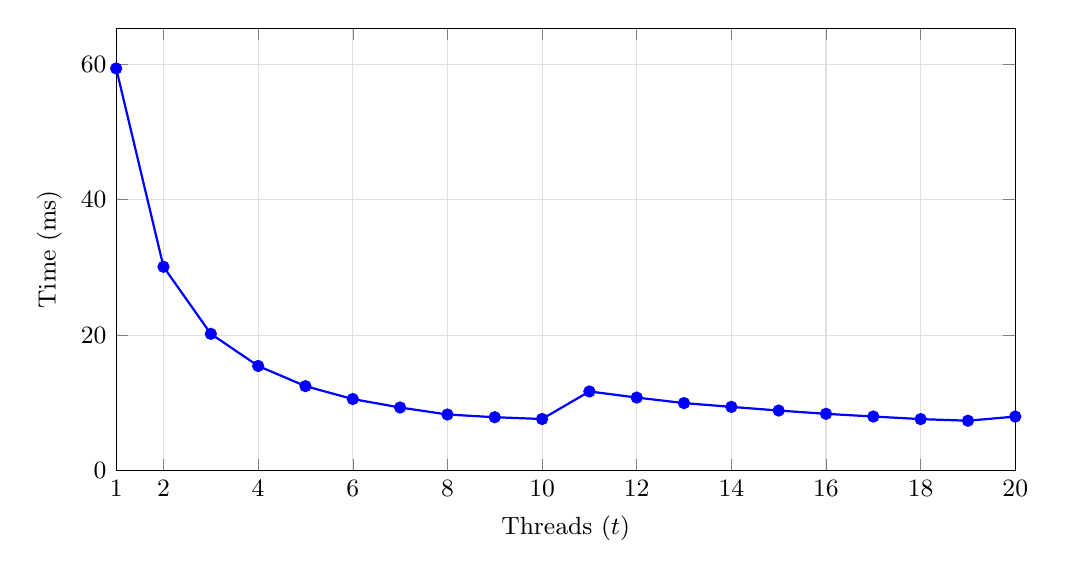
\begin{tikzpicture}
\begin{axis}[width=13cm,height=7.2cm,
xlabel={Threads ($t$)},ylabel={Time (ms)},
xmin=1,xmax=20,xtick={1,2,4,6,8,10,12,14,16,18,20},
ymin=0,grid=both,major grid style={gray!25},minor grid style={gray!10},
tick label style={font=\small},label style={font=\small},
scaled y ticks=false,/pgf/number format/1000 sep={}]
\addplot[blue,thick,mark=*,mark size=1.8pt] coordinates {
(1, 59.356959)
(2, 30.08682)
(3, 20.188375)
(4, 15.450847)
(5, 12.469043)
(6, 10.566024)
(7, 9.318026)
(8, 8.285581)
(9, 7.883735)
(10, 7.620511)
(11, 11.687551)
(12, 10.785457)
(13, 9.968445)
(14, 9.409458)
(15, 8.86755)
(16, 8.384263)
(17, 7.988066)
(18, 7.605232)
(19, 7.368248)
(20, 7.981307)
};
\end{axis}
\end{tikzpicture}
\end{document}
